%qepaper.tex
\documentclass[12pt,letterpaper]{article}
\usepackage{mathptmx}
\usepackage[margin=1in]{geometry}

\usepackage{tabularx, longtable, pdflscape, adjustbox}  % for 'tabularx' environment and 'X' column type
\usepackage{ragged2e}  % for '\RaggedRight' macro (allows hyphenation)
\newcolumntype{Y}{>{\RaggedRight\arraybackslash}X} 
\usepackage{booktabs}  % for \toprule, \midrule, and \bottomrule macros 

\usepackage{setspace}
\onehalfspacing
%\doublespacing
%\singlespacing

\usepackage{amssymb,latexsym}
\usepackage[round,sort]{natbib}
\usepackage{fancyhdr}
\usepackage{lastpage}
\usepackage{graphicx,multirow}
\graphicspath{ {qepaper/} }

% Bold Table and Figure captions
\usepackage{caption}
\captionsetup{figurename=FIGURE}
\captionsetup{tablename=TABLE}
\captionsetup[figure]{labelfont=bf}
\captionsetup[table]{labelfont=bf}

% Turns off all section numbering
\setcounter{secnumdepth}{0} 

\usepackage{titling}

  % Places all tables at end of document and creates AOM-style table-here placeholders
  \usepackage[nolists]{endfloat} % Places all figures and charts at end of manuscript and adds 'insert table x about here' lines.
  \renewcommand{\figureplace}{
    \begin{center}
    \begin{singlespace}
    ------------------------------------\\
    Insert \figurename \ \thepostfig\ about here.\\
    ------------------------------------
    \end{singlespace}
    \end{center}}
  \renewcommand{\tableplace}{%
    \begin{center}
    \begin{singlespace}
    ------------------------------------\\
    Insert \tablename \ \theposttbl\ about here.\\
    ------------------------------------
    \end{singlespace}
    \end{center}}

  \usepackage{titlesec}
   \titleformat{\title}
       {\filcenter\normalfont\bfseries\uppercase}{\thetitle}{1em}{}
  \titleformat{\section}
    {\filcenter\normalfont\bfseries\uppercase}{\thesection}{1em}{}
  \titleformat{\subsection}
    {\normalfont\bfseries}{\thesubsection}{1em}{}
  \titleformat{\subsubsection}[runin]
   {\normalfont\bfseries\slshape}{\thesubsubsection}{1em}{\hspace*{\parindent}}
       
\usepackage{tabu}
\usepackage{textcomp}
\usepackage{listings}
\usepackage{hyperref}
\usepackage{verbatim}
\usepackage{tabu}
\hypersetup{
    colorlinks=true,
    linkcolor=blue,
    filecolor=cyan,      
    urlcolor=cyan,
    citecolor=blue,
}

\usepackage{etoolbox}
\usepackage{blindtext}
\usepackage{draftwatermark}

\makeatletter

% Patch case where name and year are separated by aysep
\patchcmd{\NAT@citex}
  {\@citea\NAT@hyper@{%
     \NAT@nmfmt{\NAT@nm}%
     \hyper@natlinkbreak{\NAT@aysep\NAT@spacechar}{\@citeb\@extra@b@citeb}%
     \NAT@date}}
  {\@citea\NAT@nmfmt{\NAT@nm}%
   \NAT@aysep\NAT@spacechar\NAT@hyper@{\NAT@date}}{}{}

% Patch case where name and year are separated by opening bracket
\patchcmd{\NAT@citex}
  {\@citea\NAT@hyper@{%
     \NAT@nmfmt{\NAT@nm}%
     \hyper@natlinkbreak{\NAT@spacechar\NAT@@open\if*#1*\else#1\NAT@spacechar\fi}%
       {\@citeb\@extra@b@citeb}%
     \NAT@date}}
  {\@citea\NAT@nmfmt{\NAT@nm}%
   \NAT@spacechar\NAT@@open\if*#1*\else#1\NAT@spacechar\fi\NAT@hyper@{\NAT@date}}
  {}{}

\lstset{
basicstyle=\ttfamily,
columns=flexible,
breaklines=true
}
\newenvironment{hypothesis}{
  	\itshape
  	\leftskip=\parindent \rightskip=\parindent
  	\noindent\ignorespaces}

\fancypagestyle{plain}{
  \renewcommand{\headrulewidth}{0pt}
  \fancyhf{}
}	

\begin{document}
\SetWatermarkText{Draft}
\setlength{\droptitle}{-5em}
\title{\textbf{\large Heterogeneity in Knowledge Flows of Regions: Impact on Invention Quality}}
\date{\vspace{-12ex}}

\maketitle
\thispagestyle{empty}
\renewcommand{\abstractname}{\normalsize ABSTRACT}
\begin{abstract}
\normalsize
\noindent Using patent citations as measures of knowledge flows, we explore if the different types of knowledge flows in a region affect the quality of inventions originating in that region. We leverage a database of worldwide urban centers  obtained from remote sensing data to provide a consistent definition for regions worldwide. As some other recent research in the area \citep{todo}, our preliminary results find inconclusive evidence for a clear positive effect of local knowledge flows on invention output of regions, or the globalization of R\&D on the invention output of regions. Our work here suggests that much more research is required to distill any stylized facts on the implications of geography and firm organization on invention outcomes. 
\end{abstract}

\newpage
\pagestyle{fancy}
\fancyhf{}
\lhead{Heterogeneity in Knowledge Flows of Regions: Impact on Invention Quality}
\rhead{\thepage}

\textbf{Heterogeneity in Knowledge Flows of Regions: Impact on Invention Quality}

\vspace{3ex}


\noindent Empirical studies in the literature on economic geography have used patent citations to suggest that knowledge spillovers are geographically localized \citep*{Jaffe1993, Almeida1999, Bottazzi2003, Branstetter2001, Maurseth2002, Sonn2008}, and that innovation is more spatially concentrated that production \citep{Feldman1994a}. On the other hand, patent citations have also been used in the international business literature to demonstrate that multi-national firms (MNCs) gain from the cross-border flow of knowledge and the globalization of R\&D \citep{Singh2007, Zhao2006, Singh2013}. This leads to the question of what indeed is the net effect of geography on innovation outcomes of firms and regions. Firms seek to improve innovation outcomes as a way of building a sustainable competitive advantage. Understanding how prior knowledge flows (across firms and geographies) affect innovation outcomes would therefore be valuable to managers in their quest for superior performance. \par

In this study, we\footnote{This paper is the outcome of the joint work by my co-author and me. While the changes since the version submitted to a conference in February 2017 (sms2017.pdf, provided as supplementary material) are without consultation with my co-author, I have used the plural ``we'' throughout this paper to preserve continuity with the previous version and compatibility with future versions that are going to be jointly authored.} examine how the nature of knowledge spillovers or flows in a region affect the quality of the inventions generated in the region. Specifically, we look at knowledge flows spanning region boundaries and firm boundaries, and ask if and to what extent prior knowledge flows between and within regions and firms affects innovation quality of patents originating in a region. In this study we use citation data of patents applied for between 2001 and 2012 to empirically estimate the relationship between knowledge flows of a region and quality of inventions from that region. We are aware of no prior studies that have examined the effects of the geographical characteristics of knowledge flows on invention outcomes of regions. Our work therefore seeks to contribute to the innovation literatures in both economic geography and international business. \par 

It would seem appropriate to raise two measurement related issues here soon after we propose our research question. First, despite well known issues in the use of patents \citep{Griliches1990, Scherer1984} and in the use of patent citations to demonstrate localization of knowledge spillovers \citep*{Thompson2005, Arora2017a}, much work in understanding knowledge spillovers has continued to rely on patent citations. While our analysis in this paper is singularly dependent on data of United States patents, we are careful to not make strong assumptions about patent citations reflecting underlying knowledge flows. Wherever possible, we consider competing hypotheses built on opposing assumptions about what patent citations may capture. Second, innovations are clearly not the same as inventions. The measure of an innovation lies in its acceptance in the marketplace. An invention may therefore only represent an early event in the innovation process. While we recognize that managers and policy makers are interested in innovation outcomes, we continue to be limited by data availability that allows us to only make claims about invention quality. Despite those caveats, pursuing the questions posed above can provide not just interesting trade-offs to explore, but indeed create opportunities for a larger research agenda on actionable strategies for firms seeking to improve their innovation outcomes.\par

\textbf{Correction}
The next section reviews the theory from the geography of innovation and innovation in international business. We then define a framework to classify knowledge flows in a region and motivate our work by demonstrating how different regions fare differently in terms of knowledge flows. We build on the theory and this framework to propose our hypotheses. We then propose our research design, and follow it up with a description of our data and methods. Our preliminary results are then presented, followed by a discussion of the results. We conclude with limitations, next steps and open questions for further research.



\section*{Theory and Hypotheses}
\cite{Griliches1979} drew our attention toward two types of knowledge spillovers - ``rent spillovers" that  are rival and excludable knowledge flows that occur from the exchange of goods, and ``pure or idea-creating spillovers"  that are non-rival and non-excludable knowledge that is typically associated with R\&D activity. While rent spillovers may be characterized as a private good, pure spillovers exhibit characteristics of a public good \citep{Arrow1962}.  This dual nature of knowledge is additionally complicated by the fact that knowledge flows may be largely invisible \citep{Krugman1991a}, and only sometimes do knowledge flows leave a paper trail in the form of patent citations \citep{Jaffe1993}. In the following sections, we review the literature in economic geography and international business \textbf{Correction} cognizant of these fundamental limitations relating to the nature and measurement of knowledge.


\subsection{Economic geography of innovation}
\textbf{Correction - What is the purpose of this section}
Scholars of economics and strategy have for long recognized that clusters and agglomeration economies play an important role in fostering innovation \citep{Marshall1890, Porter1990}. Agglomeration economies may arise due to labor pooling advantages, economies of specialization of local suppliers, and knowledge spillovers \citep{Porter1990, Krugman1991a}.  Several studies have used patent citations to demonstrate that knowledge flows are localized \citep*{Jaffe1993, Almeida1999}. After controlling for the geographic distribution of production, \cite{Audretsch1996a} demonstrated that innovation exhibits a pronounced tendency to cluster spatially. \cite*{Acs1994} found that new product introductions were more geographically concentrated than patents and that they derived important inputs from universities and industrial R\&D. \par

Regions, however vary in their inventive output \citep*{Agrawal2014b} and the nature of knowledge flows in a region may be only one source of this variation within regions. Location however has been suggested to matter more at the earliest stage of the industry life cycle, with life-cycle production costs featuring more prominently in mature goods and industries. \cite{Audretsch1996b} suggest that early stages of  industry life cycles are characterized by the importance of tacit knowledge, and may hence exhibit higher a propensity to cluster to benefit from knowledge spillovers. \par

Multiple reasons have been attributed for the localized nature of knowledge spillovers. First, costs of collaboration are lower due to geographic proximity. Second, proximity has been argued to promote serendipitous and chance encounters that create the environment for new solutions. Third, diversity within a region has also been suggested to benefit innovative output \citep{Feldman1999}. Scholars have suggested that related variety \citep*{Boschma2009, Frenken2007} may benefit in the generation of new ideas and that diversity between industrial activities may benefit the transfer of ideas \citep{Jacobs1969}. Additionally, scholars have suggested that the tacit nature of knowledge, institutions and regional innovation systems may all contribute to the localization of knowledge flows  \citep{Cooke1996, Maskell1999, Howells1996, Howells2002}.

\textbf{Correction - Summarize, the reader is left hanging}
\subsection{Globalization of innovation}
Regional innovation systems have also been suggested as influencing MNC decisions to locate subsidiaries \citep{Anderson2005}. However, scholars have also considered organizational capabilities \citep{Zhao2006}, property rights, technological sourcing \citep{Florida1997}, higher product ownership and interdependence \citep{Pearce1999}, and access to highly skilled human capital. On the other hand, political borders have been found to constrain the flows of knowledge \citep{Singh2013}, but mobility of inventors helps firms improve innovation outcomes \citep*{Alnuaimi2012b}.

\textbf{Correction - Literature review is not sufficient. What is the point that you are making?}
\subsection{Inter-firm knowledge flows and geography}
The review of the literature in the economic geography and international business traditions suggests both positive and negative effects of localization of knowledge spillovers on innovation outcomes.  One the one hand agglomerations may seem to benefit firms through access to tacit knowledge, while on the other hand it may also increase the number of competitors who are specialized in the same market segment \citep{todo}. MNC subsidiary location choices seem to be affected by local factors, as well as relative ties with local firms and MNC affiliates\citep{todo}. \textbf{Correction - Write more}. In the following section, we present a simple framework with which to address this phenomenon.  

\subsection*{Effects of knowledge flows on quality of inventions}

We formalize the discussions in the previous sections by categorizing all knowledge flows incorporated into an invention along two dimensions:  first, whether the knowledge flows among inventors are local to a geographical region or not, and second, whether knowledge flows are within the boundary of the firm or not. The motivation behind defining such a structure is to both keep it simple, as well as to focus on aspects that firms and governments may have an ability to influence. Given the nuanced and subtle nature of knowledge flows, and the difficulty in measuring them, firms may be better served with simple and actionable innovation strategies \citep{todo}. \par

Our classification allows us to analyze knowledge flows in four mutually exclusive, but collectively exhaustive categories as illustrated in Figure~\ref{fig:2x2}. We next describe each quadrant and discuss how the category of knowledge flow in that quadrant can affect invention quality. Within the context of this framework, we ask what is the net effect of each category of knowledge flow on invention quality, and which category of flow has the largest effect on invention quality. \par
\begin{figure}[h!]
\begin{centering}
  \caption{Categories of knowledge flows}
  \label{fig:2x2}
  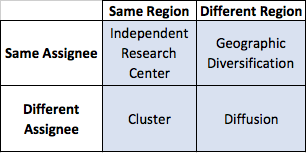
\includegraphics[width=0.8\textwidth]{2x2}
\end{centering}
\end{figure}

The top left quadrant, labelled an ``Independent Research Center" captures those knowledge flows that reflect competence building. Since these knowledge flows  are both within the region and within the firm, these flows represent local search on two dimensions (within firm and within region).  Thus, while the competence that is being built up by the Independent Research Center can be expected to have a positive effect on invention quality, the localness of the search on both dimensions may have a negative effect on invention quality. Figure~\ref{fig:SMSSameRegionSameAssigneeFlows} depicts the knowledge flows for this category (percentage of backward citations from this region that are to the same firm or assignee and same region) across time for five regions: Bangalore, Beijing, Tel Aviv-Yafo, Boston and San Jose (core of ``Silicon Valley"). While our empirical analysis covers all the major regions of the world, we chose these five regions as illustrative examples. We note that both San Jose and Boston report a higher proportion of knowledge flows within the same firm in the same region, while Bangalore and Tel Aviv-Yafo have the lowest proportion (fewer than 1\%) of their citations from the same firm within the same region. \par

\begin{figure}[h]
\begin{centering}
  \caption{Knowledge flows within regions and within assignees}
  \label{fig:SMSSameRegionSameAssigneeFlows}
  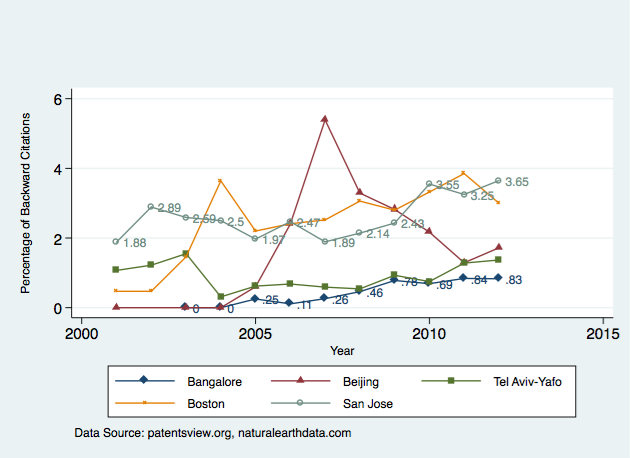
\includegraphics[width=0.90\textwidth]{SMSSameRegionSameAssigneeFlows}
\end{centering}
\end{figure}


The quadrant on the bottom left, labelled ``Cluster" captures knowledge spillovers within a region. Here firms may be seen as performing local search on one dimension (within regions) but not the other (within firms). Figure~\ref{fig:SMSSameRegionDiffAssigneeFlows} depicts the knowledge flows for this category across time for the same five regions. San Jose clearly stands out from the rest, suggesting a higher amount of across firm flows of knowledge in Silicon Valley, a result consistent with several prior studies\citep{todo}. \par

\begin{figure}[h!]
\begin{centering}
  \caption{Knowledge flows within regions and across assignees}
  \label{fig:SMSSameRegionDiffAssigneeFlows}
  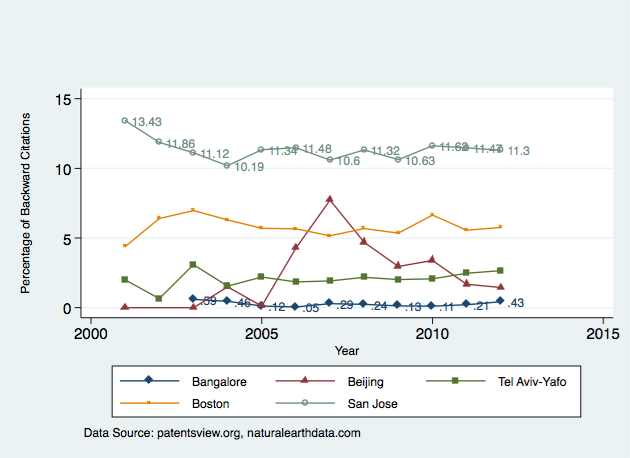
\includegraphics[width=0.90\textwidth]{SMSSameRegionDiffAssigneeFlows}
\end{centering}
\end{figure}

The quadrant on the top right, labelled as ``Geographic Diversification" captures local search on the dimension of the firm (across geographies) but not across regions. Innovations that are built on knowledge from several regions can be expected to benefit from the diversity of knowledge across regions. Yet, as in the previous quadrant, there is localness along the dimension of firm and such localness can have a negative effect on invention quality \citep{Rosenkopf2001}. Figure~\ref{fig:SMSDiffRegionSameAssigneeFlows} depicts the  knowledge flows for this category across time for the five regions. We note that Bangalore and Beijing have a relatively higher proportion of knowledge flows from same assignees in different locations, thus confirming the role of these regions as R\&D outposts of multinational firms.\par

\begin{figure}[h!]
\begin{centering}
  \caption{Knowledge flows across regions and within assignees}
  \label{fig:SMSDiffRegionSameAssigneeFlows}
  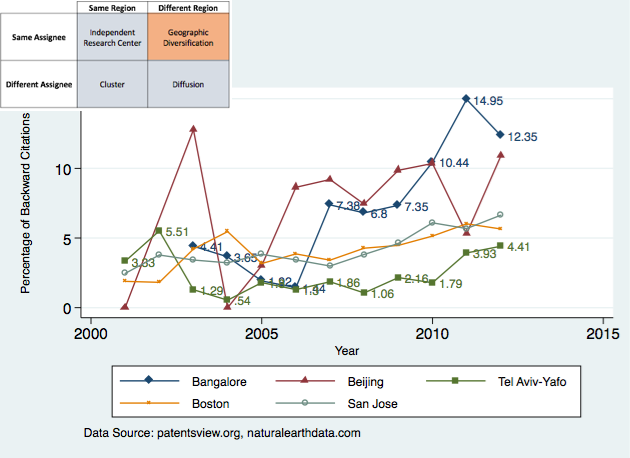
\includegraphics[width=0.90\textwidth]{SMSDiffRegionSameAssigneeFlows}
\end{centering}
\end{figure}

Finally, the bottom right quadrant labelled ``Diffusion" captures high exploration along both dimensions, indicating the development of a global pipeline \citep*{Bathelt2004}. Figure~\ref{fig:SMSDiffRegionDiffAssigneeFlows} depicts the  knowledge flows for this category across time for the five regions. We note that Bangalore, Beijing and Tel Avis-Yafo have a higher level of knowledge flows from other firms in other regions compared to Boston and San Jose, which is to be expected given that the absolute level of innovative activity in these emerging hotspots is still lower compared to that in Boston and San Jose. \par

\begin{figure}[h!]
\begin{centering}
  \caption{Knowledge flows across regions and across assignees}
  \label{fig:SMSDiffRegionDiffAssigneeFlows}
  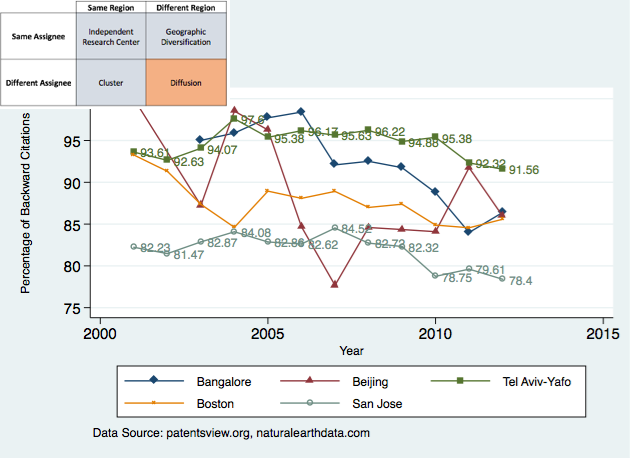
\includegraphics[width=0.90\textwidth]{SMSDiffRegionDiffAssigneeFlows}
\end{centering}
\end{figure}

As can be seen from the preceding discussion, prior theory suggests both positive and negative effects for each of these four categories of knowledge flows and it is not clear what the net effect will be on invention quality. This also suggests that prior theory does not provide guidance on which category of knowledge flows will have the highest effect on invention quality.  Since theory does not provide us with an answer, we rely on empirical analysis to inform us on the net effect of each category of knowledge flow on invention quality and which category has the highest effect on invention quality. \par


\subsubsection{Invention quality at the independent research center}
Firms operating in silos, i.e., where citations are made to other prior work within the same firm in the same region may benefit from specialization. On the other hand, the literature from economic geography suggests that related variety is associated with superior innovations  \citep{Boschma2009, Frenken2007}. It would seem, from prior literature that the cross-pollinating effect of related variety would have the larger effect on innovation outcomes\citep{todo}. \textbf{Correction - More arguments need to be provided} This leads to our first hypothesis.\\

\begin{hypothesis}
{Hypothesis 1: An increase in the proportion of same firm, same region knowledge flows will be associated with a lower level of invention quality.
\\}
\end{hypothesis}

\subsubsection{Invention quality in a cluster}
The literature on clusters suggests benefits through two different mechanisms.  Marshallian externalities are concerned with intraindustry economies of localization, while Jacobs\textquotesingle \ externalities refer to interindustry exchanges between different technologies. While some studies have suggested that Marshall-Arrow-Romer (MAR) externalities are considered more prevalent \citep{Baptista1998}, others have suggested that Jacobs\textquotesingle \ externalities dictate local knowledge spillover processes \citep{Feldman1999}. Still other studies have found both types of externalities to be significant \citep{Capello2002}. \cite*{Ibrahim2009} suggest that within metropolitan regions, the two may not be mutually exclusive. The theory therefore suggests a higher potential to generate radical, disruptive innovative output when diverse sectoral knowledge bases are combined. On the other hand, theory would suggest incremental innovation in building innovations on top of specialized knowledge \citep{Schumpeter1942}. Since a cluster itself does not lend itself to a clear definition of one type or the other, we suggest two contradictory hypotheses.\\

\begin{hypothesis}
{Hypothesis 2a: A higher proportion of different firm, same region knowledge flows to a region will be associated with a higher level of invention quality of that region\\}
\end{hypothesis}

\begin{hypothesis}
{Hypothesis 2b: A higher proportion of different firm, same region knowledge flows to a region will not be associated with a change in invention quality of that region\\}
\end{hypothesis}

\subsubsection{Invention quality under geographical diversification}
The international business literature has suggested several different effects in MNC\textquotesingle \ s structuring of R\&D across units. While agglomeration benefits have been suggested to be beneficial \citep{Cantwell2000, Nachum2000, Pantzalis2001}, scholars have also suggested potential threats from highly specialized firms in similar market niches. While the net effect on innovation under geographical diversification is not clear, innovation performance may itself only benefit. This leads to our third hypothesis.\\

\begin{hypothesis}
{Hypothesis 3: A higher proportion of same firm, different region knowledge flows to a region will be associated with a higher level of invention quality of that region\\}
\end{hypothesis}

\subsubsection{Invention quality under diffusion}
\cite{Breschi2005, Breschi2009} argue that many localized knowledge spillover studies use spatial proximity as a proxy for social proximity, and that higher innovation outcomes are determined by the access to knowledge provided by social proximity. The effect of spatial proximity itself would be greatly reduced when social proximity is accounted for. The absence of social proximity under conditions of diffusion would therefore diminish the opportunities for positive knowledge externalities. \textbf{Correction - How do you determine between no effect and negative effect}. This leads us to our final hypothesis.\\

\begin{hypothesis}
{Hypothesis 4: A higher proportion of different firm, different region knowledge flows to a region will not be associated with a change in invention quality of that region\\}
\end{hypothesis}


\section*{Data and Methods}
We use patent citations data from the U.S. Patent Office (USPTO) as provided by patentsview.org. The USPTO provides information on assignee, the location of inventors, and year of patent application. We use this information to identify which patents belong to which region in a given year. Since there can be more than one inventor on a patent, a patent can belong to more than one region. We compare the assignee and inventor location of each patent with each assignee and inventor of each backward citation  to identify the category of knowledge flow (e.g., same assignee, different location) indicated by the backward citation. Additionally, to map location data of inventors from USPTO to regions, we use urban centers data for worldwide locations from \href{http://www.naturalearthdata.com/downloads/10m-cultural-vectors/}{Natural Earth Data} that uses remote sensing data to determine urban agglomerations (a process developed in \citet*{Schneider2003}).  While it has been common practice to use Metropolitan Statistical Areas (MSA) for analyses related to economic geography in the U.S., an equivalent measure is unavailable for the rest of the world. For comparability and consistency, we choose to use the urban centers definitions from \href{http://www.naturalearthdata.com/downloads/10m-cultural-vectors/}{Natural Earth Data} for all regions both within U.S. and outside U.S. \par

Our unit of analysis is the region-year. \par

\subsection{Applicant citations and Examiner Citations}
Much of the prior work analyzing patent citations had pooled all citations made irrespective of the source (i.e., cited by applicant, or cited by examiner, or cited by other) due to lack of systematic classification of the citation source in the USPTO database. However, systematic classification of patent citations is available from 2001 onwards. Scholars have even called for more granular analysis based on citation source. For example, \cite{Alcacer2006a} suggest that inferences about inventor knowledge using pooled citations may suffer from bias or overinflated significance levels. On the other hand scholars have argued that patents cited by the examiner may not represent knowledge flows at all. To be consistent with our objective of measuring knowledge flows without strong assumptions, we do not restrict ourselves to those citations categorized as \textquotesingle cited by applicant\textquotesingle \ or those categorized as \textquotesingle cited by examiner\textquotesingle \ . We use three data sets - a) the pooled data set of all applicant and examiner citations (this is our primary data set), b) the data set of only examiner citations, and c) the data set of only applicant citations. This decision has the additional effect of limiting our period of analysis to citing patents applied for after the year 2000 since the data on which citations were added by examiners is available for patents from only 2001 onwards. 

\subsection{Citations Received}
\textbf{Correction - Revert this to counting all citations to date, and justify it}
We restrict our sample to patents applied for between 2001 - 2012, but citations received till 2015. Our default strategy for measuring patent citations is to count citations received until and including the fifth annual anniversary of the patent application. This has the effect of biasing against patent applications from 2011 and 2012.  This problem may be resolved by updating the dataset to the version updated to March 2017. For paucity of time, the dataset was not updated in time for the submission of this paper.\par

\subsection{Dependent Variable}
\textbf{Correction - Revert this to counting all citations to date, get rid of fifth annual anniversary}
Our primary dependent variable is the  total count of citations by patents belonging to a region-year. However, for all models we also report results for total non-self citations received as the dependent variable. Citations are counted as those received up to and including the fifth annual anniversary of the patent filing or until  2015, whichever is earlier. In the section on additional results, we also provide results with an alternative measure of citations received with the dataset on applicant only citations. Here we count all citations received till 2015 rather than truncate after the fifth annual anniversary of patent application filing date. 

\subsection{Independent Variables}
Building on the framework depicted in Figure ~\ref{fig:2x2}, our independent variables are the percentage of backward citations made to each of the four categories: those to a) same region, same assignee, b) same region, different assignee, c) different region, same assignee, and d) different region, same assignee. \par
\subsubsection{Percentage of backward citations made to same region and same assignee}
We compute this variable as follows. For each region, for each year, we compute the ratio of the total number of backward citations made to same region and same assignee in that year to the total number of backward citations made in that year.
\subsubsection{Percentage of backward citations made to same region and different assignee}
We compute this variable as follows. For each region, for each year, we compute the ratio of the total number of backward citations made to same region and different assignee in that year to the total number of backward citations made in that year.
\subsubsection{Percentage of backward citations made to different region and same assignee}
We compute this variable as follows. For each region, for each year, we compute the ratio of the total number of backward citations made to different region and same assignee in that year to the total number of backward citations made in that year.
\subsubsection{Percentage of backward citations made to different region and different assignee}
We compute this variable as follows. For each region, for each year, we compute the ratio of the total number of backward citations made to different region and different assignee in that year to the total number of backward citations made in that year.\par

For any given region-year, we would therefore have the sum of each of the four independent variables to add to 1 (one). \textbf{Correction - Percentage and fraction, both terminologies are used. Stick to one}

\subsection{Control Variables}
We control for the total number of citations made in the region-year, the total number of patents in the region-year, the size of the patent pool in the region-year, as well as the percentage of patents in region-year in each technology subcategory as defined by \cite*{Hall2001a}. The patent pool is the total number of patents that belong to a region up to the previous year. It is important to control for the size of the patent pool as  regions that have a larger patent pool (such as San Jose) will have more patents that can be cited and can therefore have larger within region spillovers as compared to a region that has only a small patent pool. We include region fixed effects and year dummies in all regression models so as to control for region level and year specific effects, if any. Since our dependent variable is a count variable, we use negative binomial regression analysis with fixed effects. \par

Table ~\ref{ae.corrtable} displays the correlation of our primary variables in the dataset of applicant and examiner citations. Summary statistics for the variables in the dataset of applicant and examiner citations is provided in Table ~\ref{ae.sumstat}. Similar statistics for the applicant only citations dataset and the examiner only citations dataset have been provided in the section on additional results.

\begin{center}
\begin{table}[htbp]\centering \caption{Correlation Table for Dataset of Applicant \& Examiner Citations \label{ae.corrtable}}
\scriptsize
\singlespacing
\begin{adjustbox}{angle=0}
\begin{tabular}{l  c  c  c  c  c  c  c  c  c  c }

\hline
\multicolumn{1}{c}{Variables} &1&2&3&4&5&6&7&8&9&10\\ \hline
1. Total Citations Received&1.00\\
2. Non-Self Citations Received&0.98&1.00\\
3. Self Citations Received&0.88&0.78&1.00\\
4. Share Citations Made[Same Region, Same Assignee]&0.05&0.04&0.06&1.00\\
5. Share Citations Made[Same Region, Different Assignee]&0.11&0.11&0.09&0.04&1.00\\
6. Share Citations Made[Different Region, Same Assignee]&0.00&-0.01&0.03&0.20&-0.03&1.00\\
7. Share Citations Made[Different Region, Different Assignee]&0.05&0.05&0.03&-0.22&-0.05&-0.24&1.00\\
8. Log (Total Citations Made)&0.39&0.36&0.36&0.10&0.07&0.10&0.15&1.00\\
9. Log (Num Patents)&0.31&0.29&0.27&0.12&0.14&0.04&0.18&0.83&1.00\\
10. Log (Patent Pool Size)&0.27&0.25&0.24&0.17&0.14&0.06&0.06&0.76&0.86&1.00\\ \hline
\end{tabular}
\end{adjustbox}
\end{table}
\end{center}



\begin{table}[htbp]\centering \caption{Summary Statistics for Dataset of Applicant \& Examiner Citations\label{ae.sumstat}}
\scriptsize
\singlespacing
\begin{tabular}{l c c  c}\hline\hline
\multicolumn{1}{c}{\textbf{Variable}} & \textbf{Mean}
 & \textbf{Std. Dev.} & \textbf{N}\\ \hline
Total Citations Received & 241.719 & 2063.915  & 57456\\
Non-Self Citations Received& 123.856 & 1147.495  & 57456\\
Self Citations Received& 36.581 & 360.104  & 57456\\
Share Citations Made[Same Region, Same Assignee] & 0.042 & 0.087  & 24324\\
Share Citations Made[Same Region, Different Assignee] & 0.015 & 0.05  & 24324\\
Share Citations Made[Different Region, Same Assignee] & 0.069 & 0.119  & 24324\\
Share Citations Made[Different Region, Different Assignee] & 0.444 & 0.258  & 24324\\
Log (Total Citations Made) & 3.55 & 2.237  & 24324\\
Log (Num Patents) & 2.263 & 1.94  & 57456\\
Log (Patent Pool Size) & 4.59 & 2.373  & 54716\\
\hline
\end{tabular}
\end{table}


\section*{Results}
The preliminary results from our analysis for the dataset of applicant and examiner cited patents are presented in Table~\ref{ae.model123192021}. Models 1-3 report results with the dependent variable as the total number of citations received for all regions worldwide, U.S. locations and non-U.S. locations respectively. Models 4-6 report results with the dependent variable as the number of non-self citations received. The initial observation is that results seem to vary depending on the chosen dependent variable, though the signs of the coefficients are the same. Across the models we find that knowledge flows under cluster and geographical diversification have a significant impact on the quality of inventions as measured by the number of citations received. However, the differences in the results between the two dependent variables suggests that there is an underlying effect that the current model is not capturing. \par
Let us set aside the inconsistency in results between the two measures of the dependent variable, and just focus on the results for total citations received. H1 suggested a negative effect for within firm, within region flows on invention quality. The results however suggest a positive effect and significant effect in models 1 and 3. H1 is therefore not supported. H2a and H2b suggested that potentially opposite claims for higher cluster knowledge flows. The results are mixed across the samples, suggesting perhaps that different effects are at play under different conditions. H3 predicted a positive effect for the globalized diversification driven knowledge flows. The results here are consistent with our hypotheses, across all models and across datasets. Finally, we had predicted a non-effect for the diffusion knowledge flow on invention performance. Again the results for the total citations received dependent variable hold.  \par

\begin{table}[htbp]\centering \caption{Regression Analysis of Invention Quality for Applicant \& Examiner Citations \label{ae.model123192021}}
\scriptsize
\singlespacing
\begin{tabular}{l*{6}{c}} \hline
                &\multicolumn{1}{c}{(1)}&\multicolumn{1}{c}{(2)}&\multicolumn{1}{c}{(3)}&\multicolumn{1}{c}{(4)}&\multicolumn{1}{c}{(5)}&\multicolumn{1}{c}{(6)}\\
                &\multicolumn{1}{c}{Total}&\multicolumn{1}{c}{Total}&\multicolumn{1}{c}{Total}&\multicolumn{1}{c}{Non-Self}&\multicolumn{1}{c}{Non-Self}&\multicolumn{1}{c}{Non-Self}\\
                &\multicolumn{1}{c}{Citations}&\multicolumn{1}{c}{Citations}&\multicolumn{1}{c}{Citations}&\multicolumn{1}{c}{Citations}&\multicolumn{1}{c}{Citations}&\multicolumn{1}{c}{Citations}\\
                 &\multicolumn{1}{c}{Received}&\multicolumn{1}{c}{Received}&\multicolumn{1}{c}{Received}&\multicolumn{1}{c}{Received}&\multicolumn{1}{c}{Received}&\multicolumn{1}{c}{Received}\\
\hline
Share Citations Made[Same Region, Same Assignee]&    0.211&    0.179&    0.254&    0.826&    0.899&    0.831\\
                &  (0.014)&  (0.128)&  (0.036)&  (0.000)&  (0.000)&  (0.000)\\
Share Citations Made[Same Region, Different Assignee]&   -0.393&   -0.471&  -0.0458&    0.816&    0.809&    0.811\\
                &  (0.010)&  (0.041)&  (0.808)&  (0.000)&  (0.003)&  (0.000)\\
Share Citations Made[Different Region, Same Assignee]&    0.244&    0.282&    0.326&    0.673&    0.655&    0.678\\
                &  (0.000)&  (0.002)&  (0.000)&  (0.000)&  (0.000)&  (0.000)\\
Share Citations Made[Different Region, Different Assignee]&  0.00301&   0.0243&    0.101&    0.820&    0.934&    0.802\\
                &  (0.932)&  (0.649)&  (0.036)&  (0.000)&  (0.000)&  (0.000)\\
Log (Total Citations Made)&    0.241&    0.193&    0.240&    0.180&    0.126&    0.214\\
                &  (0.000)&  (0.000)&  (0.000)&  (0.000)&  (0.000)&  (0.000)\\
Log (Num Patents)&    0.570&    0.662&    0.612&    0.634&    0.701&    0.620\\
                &  (0.000)&  (0.000)&  (0.000)&  (0.000)&  (0.000)&  (0.000)\\
Log (Patent Pool Size)&   -0.125&   -0.272&  -0.0931&  -0.0783&   -0.128&  -0.0734\\
                &  (0.000)&  (0.000)&  (0.000)&  (0.000)&  (0.000)&  (0.000)\\
Constant        &  -0.0147&    0.753&   -0.273&   -1.008&   -0.889&   -1.029\\
                &  (0.777)&  (0.000)&  (0.000)&  (0.000)&  (0.000)&  (0.000)\\
\hline
Observations    &    16111&     6449&     9662&    15701&     6324&     9377\\
Groups          &     1776&      617&     1159&     1654&      587&     1067\\
Sample&All &U.S. &Non-U.S.&All &U.S. &Non-U.S. \\
          &Locations &Locations&Locations&Locations &Locations&Locations \\
\hline\hline
\multicolumn{7}{l}{\footnotesize \textit{p}-values in parentheses}\\
\multicolumn{7}{l}{\footnotesize All regressions use negative binomial estimation on the region-year panel}\\
\multicolumn{7}{l}{\footnotesize Citations received are counted up to and including the fifth annual anniversary of a patent application}\\
\multicolumn{7}{l}{\footnotesize All models include region fixed effects, year dummies and technology subcategory controls}\\
\end{tabular}
\end{table}

\subsection{Additional Results}
Table ~\ref{e.corrtable} displays the correlation of our primary variables in the dataset of examiner only citations. Summary statistics for the variables in the dataset of examiner only citations is provided in Table ~\ref{e.sumstat}.

\begin{center}
\begin{table}[htbp]\centering \caption{Correlation Table for Dataset of Examiner Only Citations \label{e.corrtable}}
\scriptsize
\singlespacing
\begin{adjustbox}{angle=0}
\begin{tabular}{l  c  c  c  c  c  c  c  c  c  c }

\hline
\multicolumn{1}{c}{Variables} &1&2&3&4&5&6&7&8&9&10\\ \hline
1. Total Citations Received&1.00\\
2. Non-Self Citations Received&0.99&1.00\\
3. Self Citations Received&0.91&0.88&1.00\\
4. Share Citations Made[Same Region, Same Assignee]&0.04&0.03&0.06&1.00\\
5. Share Citations Made[Same Region, Different Assignee]&0.11&0.11&0.11&0.03&1.00\\
6. Share Citations Made[Different Region, Same Assignee]&-0.00&-0.01&0.02&0.23&-0.03&1.00\\
7. Share Citations Made[Different Region, Different Assignee]&0.05&0.05&0.04&-0.22&-0.05&-0.22&1.00\\
8. Log (Total Citations Made)&0.37&0.34&0.40&0.09&0.07&0.08&0.17&1.00\\
9. Log (Num Patents)&0.29&0.27&0.30&0.12&0.14&0.05&0.17&0.84&1.00\\
10. Log (Patent Pool Size)&0.25&0.23&0.26&0.17&0.13&0.05&0.06&0.75&0.86&1.00\\ \hline
\end{tabular}
\end{adjustbox}
\end{table}
\end{center}



\begin{table}[htbp]\centering \caption{Summary Statistics for Dataset of Examiner Only Citations \label{e.sumstat}}
\scriptsize
\singlespacing
\begin{tabular}{l c c  c}\hline\hline
\multicolumn{1}{c}{\textbf{Variable}} & \textbf{Mean}
 & \textbf{Std. Dev.} & \textbf{N}\\ \hline
Total Citations Received & 169.117 & 1518.954  & 57456\\
Non-Self Citations Received& 91.528 & 916.089  & 57456\\
Self Citations Received& 21.64 & 188.776  & 57456\\
Share Citations Made[Same Region, Same Assignee] & 0.042 & 0.086  & 23757\\
Share Citations Made[Same Region, Different Assignee] & 0.014 & 0.049  & 23757\\
Share Citations Made[Different Region, Same Assignee] & 0.061 & 0.111  & 23757\\
Share Citations Made[Different Region, Different Assignee] & 0.447 & 0.261  & 23757\\
Log (Total Citations Made) & 3.378 & 2.147  & 23757\\
Log (Num Patents) & 2.263 & 1.94  & 57456\\
Log (Patent Pool Size) & 4.59 & 2.373  & 54716\\
\hline
\end{tabular}
\end{table}

The additional results from our analysis for the dataset of examiner only cited patents are presented in Table~\ref{e.model123192021}. Models 1-3 report results with the dependent variable as the total number of citations received for all regions worldwide, U.S. locations and non-U.S. locations respectively. Models 4-6 report results with the dependent variable as the number of non-self citations received. The divergence between results for the two outcome measures of total citations received and non-self citations received are similar to that observed in Table~\ref{ae.model123192021} on the dataset with applicant and examiner citations. \par

\begin{table}[htbp]\centering \caption{Regression Analysis of Invention Quality for Examiner Only Citations \label{e.model123192021}}
\scriptsize
\singlespacing
\begin{tabular}{l*{6}{c}} \hline
                &\multicolumn{1}{c}{(1)}&\multicolumn{1}{c}{(2)}&\multicolumn{1}{c}{(3)}&\multicolumn{1}{c}{(4)}&\multicolumn{1}{c}{(5)}&\multicolumn{1}{c}{(6)}\\
                &\multicolumn{1}{c}{Total}&\multicolumn{1}{c}{Total}&\multicolumn{1}{c}{Total}&\multicolumn{1}{c}{Non-Self}&\multicolumn{1}{c}{Non-Self}&\multicolumn{1}{c}{Non-Self}\\
                &\multicolumn{1}{c}{Citations}&\multicolumn{1}{c}{Citations}&\multicolumn{1}{c}{Citations}&\multicolumn{1}{c}{Citations}&\multicolumn{1}{c}{Citations}&\multicolumn{1}{c}{Citations}\\
                 &\multicolumn{1}{c}{Received}&\multicolumn{1}{c}{Received}&\multicolumn{1}{c}{Received}&\multicolumn{1}{c}{Received}&\multicolumn{1}{c}{Received}&\multicolumn{1}{c}{Received}\\
\hline
Share Citations Made[Same Region, Same Assignee]&    0.289&    0.151&    0.437&    0.929&    0.981&    0.925\\
                &  (0.000)&  (0.168)&  (0.000)&  (0.000)&  (0.000)&  (0.000)\\
Share Citations Made[Same Region, Different Assignee]&    0.279&  -0.0690&    0.510&    1.278&    0.765&    1.358\\
                &  (0.059)&  (0.756)&  (0.009)&  (0.000)&  (0.009)&  (0.000)\\
Share Citations Made[Different Region, Same Assignee]&    0.169&   0.0516&    0.270&    0.662&    0.446&    0.777\\
                &  (0.007)&  (0.571)&  (0.002)&  (0.000)&  (0.000)&  (0.000)\\
Share Citations Made[Different Region, Different Assignee]&   0.0489&   0.0463&    0.135&    0.961&    1.100&    0.907\\
                &  (0.156)&  (0.346)&  (0.005)&  (0.000)&  (0.000)&  (0.000)\\
Log (Total Citations Made)&    0.377&    0.331&    0.395&    0.410&    0.367&    0.430\\
                &  (0.000)&  (0.000)&  (0.000)&  (0.000)&  (0.000)&  (0.000)\\
Log (Num Patents)&    0.479&    0.552&    0.500&    0.433&    0.483&    0.448\\
                &  (0.000)&  (0.000)&  (0.000)&  (0.000)&  (0.000)&  (0.000)\\
Log (Patent Pool Size)&   -0.112&   -0.236&   -0.113&  -0.0856&   -0.141&  -0.0999\\
                &  (0.000)&  (0.000)&  (0.000)&  (0.000)&  (0.000)&  (0.000)\\
Constant        &    0.409&    1.230&    0.169&   -0.688&   -0.441&   -0.688\\
                &  (0.000)&  (0.000)&  (0.010)&  (0.000)&  (0.001)&  (0.000)\\
\hline
Observations    &    15760&     6362&     9398&    15345&     6225&     9120\\
Groups          &     1738&      611&     1127&     1619&      581&     1038\\
Sample&All &U.S. &Non-U.S.&All &U.S. &Non-U.S. \\
          &Locations &Locations&Locations&Locations &Locations&Locations \\
\hline\hline
\multicolumn{7}{l}{\footnotesize \textit{p}-values in parentheses}\\
\multicolumn{7}{l}{\footnotesize All regressions use negative binomial estimation on the region-year panel}\\
\multicolumn{7}{l}{\footnotesize Citations received are counted up to and including the fifth annual anniversary of a patent application}\\
\multicolumn{7}{l}{\footnotesize All models include region fixed effects, year dummies and technology subcategory controls}\\
\end{tabular}
\end{table}


Table ~\ref{a.tcorrtable} displays the correlation of our primary variables in the dataset of applicant only citations. Summary statistics for the variables in the dataset of applicant only citations is provided in Table ~\ref{a.tsumstat}.

\begin{table}[htbp]\centering \caption{Correlation table for applicant only data set with dependent variable as total citations received \label{a.tcorrelation}}
\begin{tabular}{l  c  c  c  c  c  c  c  c  c  c  c  c }\hline\hline
\multicolumn{1}{c}{Variables} &Total Citations Received&Non-Self Citations Received&Self Citations Received&Share Citations Made[Same Region, Same Assignee]&Share Citations Made[Same Region, Different Assignee]&Share Citations Made[Different Region, Same Assignee]&Share Citations Made[Different Region, Different Assignee]&Share Citations Made[Same Region]&Share Citations Made[Same Assignee]&Log (Total Citations Made)&Log (Num Patents)&Log (Patent Pool Size)\\ \hline
Total Citations Received&1.00\\
Non-Self Citations Received&0.99&1.00\\
Self Citations Received&0.79&0.70&1.00\\
Share Citations Made[Same Region, Same Assignee]&0.05&0.04&0.08&1.00\\
Share Citations Made[Same Region, Different Assignee]&0.14&0.13&0.13&0.09&1.00\\
Share Citations Made[Different Region, Same Assignee]&-0.02&-0.02&0.01&0.18&-0.04&1.00\\
Share Citations Made[Different Region, Different Assignee]&-0.04&-0.04&-0.07&-0.49&-0.32&-0.88&1.00\\
Share Citations Made[Same Region]&0.13&0.12&0.14&0.72&0.75&0.09&-0.55&1.00\\
Share Citations Made[Same Assignee]&-0.00&-0.01&0.03&0.49&-0.01&0.95&-0.95&0.32&1.00\\
Log (Total Citations Made)&0.27&0.24&0.33&0.11&0.12&0.07&-0.13&0.15&0.10&1.00\\
Log (Num Patents)&0.38&0.36&0.36&0.14&0.16&0.01&-0.11&0.20&0.06&0.72&1.00\\
Log (Patent Pool Size)&0.34&0.32&0.33&0.15&0.19&0.01&-0.12&0.23&0.06&0.71&0.94&1.00\\
\hline \hline 
 \end{tabular}
\end{table}


\begin{table}[htbp]\centering \caption{Summary statistics for applicant only data set with DV as Total Citations Received (distance calculated) \label{a.tsummary}}
\scriptsize
\singlespacing
\begin{tabular}{l c c  c}\hline\hline
\multicolumn{1}{c}{\textbf{Variable}} & \textbf{Mean}
 & \textbf{Std. Dev.} & \textbf{N}\\ \hline
Total Citations Received & 1762.906 & 8670.540  & 8947\\
Non-Self Citations Received & 1423.084 & 7358.189  & 8947\\
Self Citations Received & 339.822 & 1754.63  & 8947\\
Share Citations Made[Same Region, Same Assignee] & 0.016 & 0.042  & 8947\\
Share Citations Made[Same Region, Different Assignee] & 0.016 & 0.045  & 8947\\
Share Citations Made[Different Region, Same Assignee] & 0.065 & 0.11  & 8947\\
Share Citations Made[Different Region, Different Assignee] & 0.903 & 0.132  & 8947\\
Share Citations Made[Same Region] & 0.032 & 0.064  & 8947\\
Share Citations Made[Same Assignee] & 0.081 & 0.125  & 8947\\
Log (Total Citations Made) & 4.891 & 2.397  & 8947\\
Log (Num Patents) & 3.807 & 1.928  & 8947\\
Log (Patent Pool Size) & 6.586 & 2.02  & 8947\\
\hline\end{tabular}
\end{table}



GITCRYPT�m�X!)^	!?�t��-�J�o�ڠ��I�vA�O��C	�"�}ǯ�@����*]������.�1^�);�p>��zc�s^��#jw(^�u-H<�4���xt
6��BM̀�"�}h��e� r��
ReIŒV>3��d+�I���4�O*�Y�R���4wT�sœ"�?x���\�S����%<����Y�ՔD6���+�Ce':�ˡj��E��HO/���{��)-��I
����o�ڳj58N!㈩�/��Aj�-�d㾡�(k����mĄ�cy���`�K����w��G�
��RoA���r����Q:�P�`�F�3k��
x�|H����5'`�/]X�7�L����?x����w�E�aP�Fj����]����:��}�	z*Zpf�c)D�����ٲh��_��!�ar��٠K�f��6չ?Out��C�]��R�\k��Ճ�����s��W>�EE���Z�"�
��~ߜKp��,�A��^c�����ߒ���ԼSm������A}�sR��pX3��b�z��ӧ	��]£`/��B�#�)�����d��[���ϬvX
�� �}��tw�����y#W���4���w�U�xyBL�A�y�����m�ԛ`��Y��U��Ʋ��6��޻�spI��w�EV��Q�E|WB�ZlZ6,��HI��_�I+n�
ISg�J�Of]ts��*3�t36�}}�rs��t{�N��!�R�����j�8�Ø�ܭ�R�=3�#�����#Pk�]ST�i�L�Y�L*�R�C�Ӊ�(3�@-�c3AD�P�g`�Fݍ*C����
�7"Z�n[��z�?u{�+qa���l]��rj�%��4�0�?��*Gp=��r��J�^	��\
|�)4шS�C��($���|�`zՐ�<�fX�

�B�Qrw��b3�{��y5ݤY"�i�{��Y���
+2�.ƍ�j���� �s�%��Ԏ쇗#1X�3�O����m���m�Ut�9?_���ve���?3 �6�{�0��(�	Y~�{VП*��P�x7�RAkዴ�
�s�;T��p��ɝDּ��آvREb���
[g�c��b��iO��D��RJ_�����^po*��C�;bz�)��D~�FaX��^��l�&,��_��tg<Z�(�,����Ո�p��x[�ks锅��B�7�f
o�z��1ƌ��2����V��b'�lئ0�K�o����Va>a����A�<EE�9��9�.��u�l�ּ��c�z���&z.��@��0����������7�w�nX'´,�t�z)e%P:㡳ɕVϽ�J��<�m��p�_㒰�MQ����~Xe�е��ߞ��F��|���K��I�Dd%��.��K���.]`V@$[#,K+���%�y����:=I�0Cl�4f 9���<Ml�A�:�	"�w�_����+gFA����e��!���8ƍh��e:��\���35��H�\d|귚@�6&?�*���2c��dV�*�%:%�rQf����w�v��%����D�}-*���|K�y���5-��v��V��ݪ�1:\$&ceZ�I�y�b���;��k/a��p��.���*���

\begin{table}[htbp]\centering \caption{Summary statistics for applicant only data set with DV as Non-Self Citations Received (distance calculated) \label{a.nsummary}}
\begin{tabular}{l c c  c}\hline\hline
\multicolumn{1}{c}{\textbf{Variable}} & \textbf{Mean}
 & \textbf{Std. Dev.} & \textbf{N}\\ \hline
Total Citations Received & 1780.181 & 8711.249  & 8860\\
Non-Self Citations Received & 1437.058 & 7392.873  & 8860\\
Self Citations Received & 343.123 & 1762.906  & 8860\\
Share Citations Made[Same Region, Same Assignee] & 0.016 & 0.042  & 8860\\
Share Citations Made[Same Region, Different Assignee] & 0.017 & 0.044  & 8860\\
Share Citations Made[Different Region, Same Assignee] & 0.065 & 0.108  & 8860\\
Share Citations Made[Different Region, Different Assignee] & 0.903 & 0.131  & 8860\\
Share Citations Made[Other] & 0 & 0  & 8860\\
Share Citations Made[Same Region] & 0.032 & 0.064  & 8860\\
Share Citations Made[Same Assignee] & 0.08 & 0.123  & 8860\\
Log (Total Citations Made) & 4.914 & 2.394  & 8860\\
Log (Num Patents) & 3.836 & 1.913  & 8860\\
Log (Patent Pool Size) & 6.622 & 1.993  & 8860\\
\hline\end{tabular}
\end{table}


The additional results from our analysis for the dataset of applicant only cited patents are presented in Table~\ref{a.model123192021}. Models 1-3 report results with the dependent variable as the total number of citations received for all regions worldwide, U.S. locations and non-U.S. locations respectively. Models 4-6 report results with the dependent variable as the number of non-self citations received. The divergence between results for the two outcome measures of total citations received and non-self citations received are similar to that observed in Table~\ref{ae.model123192021} on the dataset with applicant and examiner citations. \par

\begin{table}[htbp]\centering \caption{Regression Analysis of Invention Quality for Applicant Citations Only \label{a.model123192021}}
\scriptsize
\singlespacing
\begin{tabular}{l*{6}{c}} \hline
                &\multicolumn{1}{c}{(1)}&\multicolumn{1}{c}{(2)}&\multicolumn{1}{c}{(3)}&\multicolumn{1}{c}{(4)}&\multicolumn{1}{c}{(5)}&\multicolumn{1}{c}{(6)}\\
                &\multicolumn{1}{c}{Total}&\multicolumn{1}{c}{Total}&\multicolumn{1}{c}{Total}&\multicolumn{1}{c}{Non-Self}&\multicolumn{1}{c}{Non-Self}&\multicolumn{1}{c}{Non-Self}\\
                &\multicolumn{1}{c}{Citations}&\multicolumn{1}{c}{Citations}&\multicolumn{1}{c}{Citations}&\multicolumn{1}{c}{Citations}&\multicolumn{1}{c}{Citations}&\multicolumn{1}{c}{Citations}\\
                 &\multicolumn{1}{c}{Received}&\multicolumn{1}{c}{Received}&\multicolumn{1}{c}{Received}&\multicolumn{1}{c}{Received}&\multicolumn{1}{c}{Received}&\multicolumn{1}{c}{Received}\\
\hline
Share Citations Made[Same Region, Same Assignee]&   -0.125&   -0.150&  -0.0872&   -0.256&   -0.302&   -0.240\\
                &  (0.184)&  (0.290)&  (0.490)&  (0.017)&  (0.065)&  (0.100)\\
Share Citations Made[Same Region, Different Assignee]&   -0.229&   -0.281&  -0.0944&    0.252&    0.222&    0.253\\
                &  (0.116)&  (0.245)&  (0.599)&  (0.097)&  (0.393)&  (0.187)\\
Share Citations Made[Different Region, Same Assignee]&    0.114&    0.217&   0.0820&   0.0375&    0.109&  -0.0360\\
                &  (0.080)&  (0.023)&  (0.364)&  (0.622)&  (0.326)&  (0.733)\\
Share Citations Made[Different Region, Different Assignee]&  -0.0703&  -0.0400&  -0.0725&  -0.0220&   0.0199&  -0.0546\\
                &  (0.107)&  (0.535)&  (0.221)&  (0.647)&  (0.782)&  (0.405)\\
Log (Total Citations Made)&   0.0556&   0.0464&   0.0596&   0.0378&   0.0210&   0.0423\\
                &  (0.000)&  (0.000)&  (0.000)&  (0.000)&  (0.030)&  (0.000)\\
Log (Num Patents)&    0.712&    0.780&    0.700&    0.720&    0.768&    0.743\\
                &  (0.000)&  (0.000)&  (0.000)&  (0.000)&  (0.000)&  (0.000)\\
Log (Patent Pool Size)&  -0.0436&   -0.153&  0.00211&   0.0188&  -0.0287&-0.0000276\\
                &  (0.075)&  (0.000)&  (0.950)&  (0.509)&  (0.542)&  (0.999)\\
Constant        &   -2.621&   -2.141&   -2.944&   -3.255&   -2.997&   -3.380\\
                &  (0.000)&  (0.000)&  (0.000)&  (0.000)&  (0.000)&  (0.000)\\
\hline
Observations    &     7275&     3434&     3841&     7080&     3357&     3723\\
Groups          &     1095&      483&      612&     1019&      454&      565\\
Sample&All &U.S. &Non-U.S.&All &U.S. &Non-U.S. \\
          &Locations &Locations&Locations&Locations &Locations&Locations \\
\hline\hline
\multicolumn{7}{l}{\footnotesize \textit{p}-values in parentheses}\\
\multicolumn{7}{l}{\footnotesize All regressions use negative binomial estimation on the region-year panel}\\
\multicolumn{7}{l}{\footnotesize All models include region fixed effects, year dummies and technology subcategory controls}\\
\end{tabular}
\end{table}



The additional results from our analysis for the dataset of applicant only cited patents with citations received counted till 2015 are presented in Table~\ref{ainf.model123192021}. Models 1-3 report results with the dependent variable as the total number of citations received for all regions worldwide, U.S. locations and non-U.S. locations respectively. Models 4-6 report results with the dependent variable as the number of non-self citations received. Interestingly here, we note that results between the two dependent variable measures are not particularly different. However, these set of measures seem to suggest different effects to that observed in Table~\ref{a.model123192021} on the dataset with applicant only citations but where citations were counted until the fifth annual anniversary of the patent filing date. This suggests that we may need to investigate the time effect on citations more closely. \par

\begin{table}[htbp]\centering \caption{Regression Analysis of Invention Quality* for Applicant Only Citations  \label{ainf.model123192021}}
\scriptsize
\singlespacing
\begin{tabular}{l*{6}{c}} \hline
                &\multicolumn{1}{c}{(1)}&\multicolumn{1}{c}{(2)}&\multicolumn{1}{c}{(3)}&\multicolumn{1}{c}{(4)}&\multicolumn{1}{c}{(5)}&\multicolumn{1}{c}{(6)}\\
                &\multicolumn{1}{c}{Total}&\multicolumn{1}{c}{Total}&\multicolumn{1}{c}{Total}&\multicolumn{1}{c}{Non-Self}&\multicolumn{1}{c}{Non-Self}&\multicolumn{1}{c}{Non-Self}\\
                &\multicolumn{1}{c}{Citations}&\multicolumn{1}{c}{Citations}&\multicolumn{1}{c}{Citations}&\multicolumn{1}{c}{Citations}&\multicolumn{1}{c}{Citations}&\multicolumn{1}{c}{Citations}\\
                 &\multicolumn{1}{c}{Received}&\multicolumn{1}{c}{Received}&\multicolumn{1}{c}{Received}&\multicolumn{1}{c}{Received}&\multicolumn{1}{c}{Received}&\multicolumn{1}{c}{Received}\\
\hline
Share Citations Made[Same Region, Same Assignee]&   -0.169         &   -0.104         &   -0.134&-0.232         &   -0.183         &   -0.316 \\
                &   (0.218)         &  (0.623)         &  (0.454)&   (0.105)         &  (0.392)         &  (0.123) \\
Share Citations Made[Same Region, Different Assignee]&    -0.149         &   -0.191         &  -0.0919&    0.0391         &   0.0945         &   0.0505 \\
                &   (0.215)         &  (0.458)         &  (0.468) &   (0.733)         &  (0.721)         &  (0.699) \\
Share Citations Made[Different Region, Same Assignee]&     0.217  &    0.266  &    0.348&    0.195  &    0.263  &    0.174 \\
                &(0.012)         &  (0.037)         &  (0.004) &   (0.035)         &  (0.041)         &  (0.212)\\
Share Citations Made[Different Region, Different Assignee]&  0.00828         &   0.0315         &   0.0179&   0.00989         &   0.0203         &  0.00983  \\
                &  (0.789)         &  (0.499)         &  (0.661)&    (0.762)         &  (0.675)         &  (0.826)         \\
Log (Total Citations Made)&    0.0180&   0.0198&   0.0134&     0.0150&   0.0139  &   0.0107 \\
                &   (0.000)         &  (0.001)         &  (0.014)&   (0.000)         &  (0.023)         &  (0.075) \\
Log (Num Patents)&     0.785&    0.811&    0.830&        0.772&    0.795&    0.828\\
                &  (0.000)         &  (0.000)         &  (0.000)&  (0.000)&  (0.000)&  (0.000)\\
Log (Patent Pool Size)&  -0.111&   -0.227&  -0.0944&    -0.0453  &   -0.108 &  -0.0685\\
                &  (0.075)&  (0.000)&  (0.950)&   (0.039)         &  (0.006)         &  (0.017) \\
\hline
Observations    &    9241&3885&5356&          8879         &     3732         &     5147\\
Groups          &     1314&529&785&1199         &      478         &      721\\
Sample&All &U.S. &Non-U.S.&All &U.S. &Non-U.S. \\
          &Locations &Locations&Locations&Locations &Locations&Locations \\
\hline\hline
\multicolumn{7}{l}{\footnotesize \textit{p}-values in parentheses}\\
\multicolumn{7}{l}{\footnotesize All regressions use negative binomial estimation on the region-year panel}\\
\multicolumn{7}{l}{\footnotesize * Citations received are counted all the way to end 2016 for which data is available}\\
\multicolumn{7}{l}{\footnotesize All models include region fixed effects, year dummies and technology subcategory controls}\\
\end{tabular}
\end{table}


\section*{Discussion}
Knowledge flows are hard to measure, and knowledge is characterized by by opposing qualities of being tacit and coded, and of behaving like a public or a private good. The central challenge therefore seems to be to find a way to disentangle the opposing natures of knowledge. It is possibly this that is behind the different results we observe between the two dependent variable measures of total citations received and non-self citations received. In fact, the 2005 debate in the American Economic Review highlights how minor changes in measures can dramatically alter results when measuring knowledge and its effects \citep*{Henderson2005, Thompson2005}. The question then is if there is an alternative means to measure knowledge flows more reliably, or if the problem lies with the research methodology used herein. \cite{Maurseth2002} have suggested a regional compatibility index for capturing technological linkages. An alternate approach of understanding knowledge flows relies on the movement of people with the assumption that knowledge is embedded within an individual. While patent citations arguably mapped codified knowledge, mobility captures a measure of tacit knowledge \citep{Polanyi1958}. However even in this tradition, scholars have suggested opposite effects of knowledge flows. While \cite{Almeida1997} show that mobility patterns of star inventors directly the geographic patterns of knowledge spillovers, \cite{Song2003} illustrate that mobile engineers who join a firm with stronger path dependence are unlikely to build on the knowledge of their previous firms. While geography may be seen as providing a platform to organize these interactions amongst inventors, it seems that we may need to consider other dimensions of geography so as to fully understand the effect on invention outcomes \citep{Bunnell2001}. Universities, research consortia, and other institutions may play a significant role in affecting invention outcomes.

\section*{Limitations}
In addition to the customary disclaimers about using patent citations as measures of knowledge flows, we would like to highlight a couple of limitations that may stem from the methodology we adopted. While the use of patent citations as a measure of knowledge flows has been popular in the literature, this may nevertheless be subject to error \citep*{Arora2017a}. Our definition of regions is dependent on the latitude/longitude assignment in the patentsview.org data and on the urban centers definition in the \href{http://www.naturalearthdata.com/downloads/10m-cultural-vectors/}{Natural Earth Data}. Any systematic biases in the definition of regions can create biases in measures of within region and across region knowledge flows. \par

\section*{Conclusion}
While still at a preliminary stage, our analysis seem to suggest that knowledge flows are extremely sensitive to the nature of mesurement deployed. This casts a doubt on the widely accepted idea that local knowledge spillovers are an important source of agglomeration economies. On the other, it also brings us to bear on the important issue of measuring knowledge flows. A potential extension of the study could be to conduct empirical analysis at the level of firm-year rather than at the region-year. We could additionally look at the additional dimension of technology (within and outside technological domain, \cite{Rosenkopf2001}) in addition to those of within/outside region and within/outside firm. This may provide us with a more nuanced understanding of the factors affecting invention quality. Future studies could potentially examine other measures of invention outcomes such as breakthrough inventions. Finally, while our work suggests multiple effects of knowledge flows on invention quality, it is not quite as clear why this may be the case. We have attempted to provide some direction by building from the theory on both streams economic geography, and international business, but there is clearly a lot to be done. We hope that our current work spurs further research in this direction.  

%\onehalfspacing
%\singlespacing
\renewcommand{\refname}{REFERENCES}
\singlespacing
\bibliography{/Users/aiyenggar/code/bibliography/aiyenggar} 
\bibliographystyle{ai-amjlike}
\newpage
%\normalsize

\end{document}
